% Figure 1 of the technical report, written by scripts/paper-figures.py from the same
% ROWS as site/public/paper/figure-1.svg. Do not edit: run the script again.
\definecolor{paperfigblue}{HTML}{0284C7}
\definecolor{paperfigorange}{HTML}{C2410C}
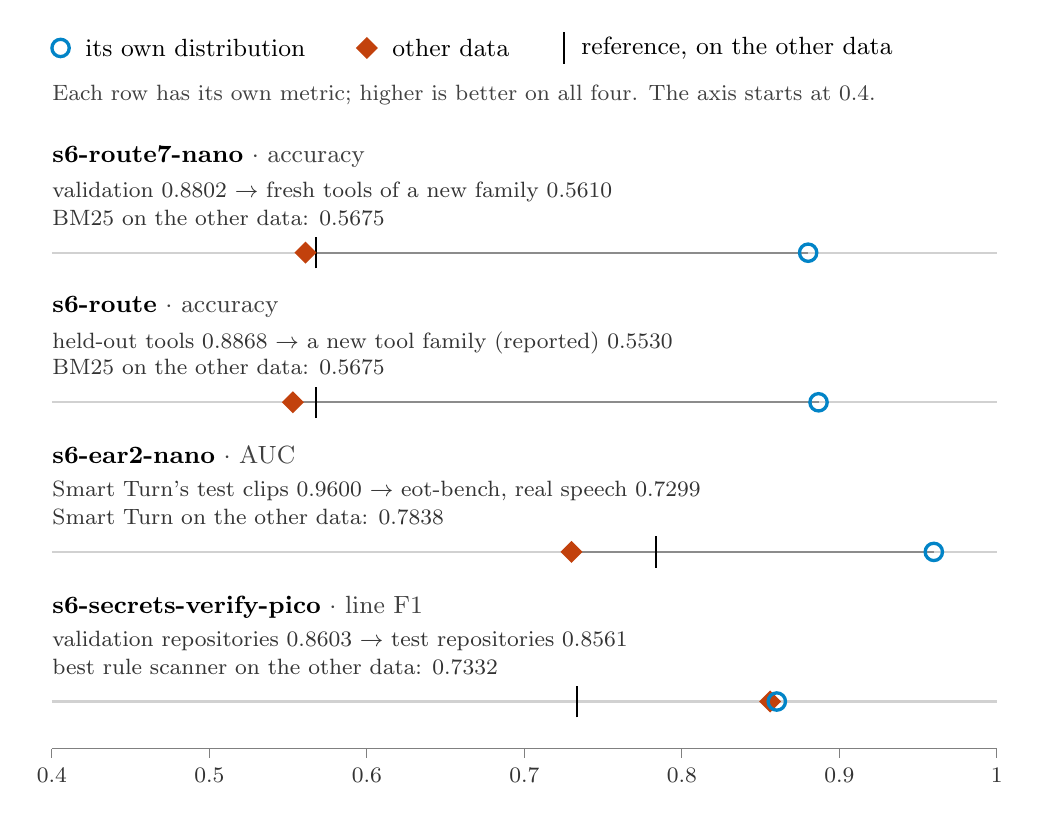
\begin{tikzpicture}[x=1cm,y=1cm,font=\small]
\draw[paperfigblue,line width=1.2pt] (0.11,0) circle (0.11);
\node[anchor=west] at (0.3,0) {its own distribution};
\fill[paperfigorange] (4.000,0.140) -- (4.140,0.000) -- (4.000,-0.140) -- (3.860,0.000) -- cycle;
\node[anchor=west] at (4.2,0) {other data};
\draw[line width=0.8pt] (6.5,-0.2) -- (6.5,0.2);
\node[anchor=west] at (6.6,0) {reference, on the other data};
\node[anchor=west,inner sep=0pt,text=black!75,font=\footnotesize] at (0,-0.6) {Each row has its own metric; higher is better on all four. The axis starts at 0.4.};
\node[anchor=north west,inner sep=0pt] at (0,-1.250) {\textbf{s6-route7-nano}\textcolor{black!75}{~$\cdot$~accuracy}};
\node[anchor=north west,inner sep=0pt,text=black!80,font=\footnotesize] at (0,-1.700) {validation 0.8802 $\rightarrow$ fresh tools of a new family 0.5610};
\node[anchor=north west,inner sep=0pt,text=black!80,font=\footnotesize] at (0,-2.050) {BM25 on the other data: 0.5675};
\draw[black!18,line width=0.8pt] (0,-2.600) -- (12.000,-2.600);
\draw[black!45,line width=0.8pt] (3.220,-2.600) -- (9.604,-2.600);
\draw[line width=0.8pt] (3.350,-2.800) -- (3.350,-2.400);
\fill[paperfigorange] (3.220,-2.460) -- (3.360,-2.600) -- (3.220,-2.740) -- (3.080,-2.600) -- cycle;
\draw[paperfigblue,line width=1.2pt] (9.604,-2.600) circle (0.11);
\node[anchor=north west,inner sep=0pt] at (0,-3.150) {\textbf{s6-route}\textcolor{black!75}{~$\cdot$~accuracy}};
\node[anchor=north west,inner sep=0pt,text=black!80,font=\footnotesize] at (0,-3.600) {held-out tools 0.8868 $\rightarrow$ a new tool family (reported) 0.5530};
\node[anchor=north west,inner sep=0pt,text=black!80,font=\footnotesize] at (0,-3.950) {BM25 on the other data: 0.5675};
\draw[black!18,line width=0.8pt] (0,-4.500) -- (12.000,-4.500);
\draw[black!45,line width=0.8pt] (3.060,-4.500) -- (9.736,-4.500);
\draw[line width=0.8pt] (3.350,-4.700) -- (3.350,-4.300);
\fill[paperfigorange] (3.060,-4.360) -- (3.200,-4.500) -- (3.060,-4.640) -- (2.920,-4.500) -- cycle;
\draw[paperfigblue,line width=1.2pt] (9.736,-4.500) circle (0.11);
\node[anchor=north west,inner sep=0pt] at (0,-5.050) {\textbf{s6-ear2-nano}\textcolor{black!75}{~$\cdot$~AUC}};
\node[anchor=north west,inner sep=0pt,text=black!80,font=\footnotesize] at (0,-5.500) {Smart Turn's test clips 0.9600 $\rightarrow$ eot-bench, real speech 0.7299};
\node[anchor=north west,inner sep=0pt,text=black!80,font=\footnotesize] at (0,-5.850) {Smart Turn on the other data: 0.7838};
\draw[black!18,line width=0.8pt] (0,-6.400) -- (12.000,-6.400);
\draw[black!45,line width=0.8pt] (6.598,-6.400) -- (11.200,-6.400);
\draw[line width=0.8pt] (7.676,-6.600) -- (7.676,-6.200);
\fill[paperfigorange] (6.598,-6.260) -- (6.738,-6.400) -- (6.598,-6.540) -- (6.458,-6.400) -- cycle;
\draw[paperfigblue,line width=1.2pt] (11.200,-6.400) circle (0.11);
\node[anchor=north west,inner sep=0pt] at (0,-6.950) {\textbf{s6-secrets-verify-pico}\textcolor{black!75}{~$\cdot$~line F1}};
\node[anchor=north west,inner sep=0pt,text=black!80,font=\footnotesize] at (0,-7.400) {validation repositories 0.8603 $\rightarrow$ test repositories 0.8561};
\node[anchor=north west,inner sep=0pt,text=black!80,font=\footnotesize] at (0,-7.750) {best rule scanner on the other data: 0.7332};
\draw[black!18,line width=0.8pt] (0,-8.300) -- (12.000,-8.300);
\draw[black!45,line width=0.8pt] (9.122,-8.300) -- (9.206,-8.300);
\draw[line width=0.8pt] (6.664,-8.500) -- (6.664,-8.100);
\fill[paperfigorange] (9.122,-8.160) -- (9.262,-8.300) -- (9.122,-8.440) -- (8.982,-8.300) -- cycle;
\draw[paperfigblue,line width=1.2pt] (9.206,-8.300) circle (0.11);
\draw[black!50] (0,-8.900) -- (12.000,-8.900);
\draw[black!50] (0.000,-8.900) -- (0.000,-9.020) node[below,text=black!80,font=\footnotesize] {0.4};
\draw[black!50] (2.000,-8.900) -- (2.000,-9.020) node[below,text=black!80,font=\footnotesize] {0.5};
\draw[black!50] (4.000,-8.900) -- (4.000,-9.020) node[below,text=black!80,font=\footnotesize] {0.6};
\draw[black!50] (6.000,-8.900) -- (6.000,-9.020) node[below,text=black!80,font=\footnotesize] {0.7};
\draw[black!50] (8.000,-8.900) -- (8.000,-9.020) node[below,text=black!80,font=\footnotesize] {0.8};
\draw[black!50] (10.000,-8.900) -- (10.000,-9.020) node[below,text=black!80,font=\footnotesize] {0.9};
\draw[black!50] (12.000,-8.900) -- (12.000,-9.020) node[below,text=black!80,font=\footnotesize] {1};
\end{tikzpicture}
